\documentclass[12pt, titlepage]{article}

\usepackage{fullpage}
\usepackage[round]{natbib}
\usepackage{multirow}
\usepackage{booktabs}
\usepackage{tabularx}
\usepackage{graphicx}
\usepackage{float}
\usepackage{hyperref}
\hypersetup{
    colorlinks,
    citecolor=blue,
    filecolor=black,
    linkcolor=red,
    urlcolor=blue
}

%% Comments

\usepackage{color}

\newif\ifcomments\commentstrue %displays comments
%\newif\ifcomments\commentsfalse %so that comments do not display

\ifcomments
\newcommand{\authornote}[3]{\textcolor{#1}{[#3 ---#2]}}
\newcommand{\todo}[1]{\textcolor{red}{[TODO: #1]}}
\else
\newcommand{\authornote}[3]{}
\newcommand{\todo}[1]{}
\fi

\newcommand{\wss}[1]{\authornote{blue}{SS}{#1}} 
\newcommand{\plt}[1]{\authornote{magenta}{TPLT}{#1}} %For explanation of the template
\newcommand{\an}[1]{\authornote{cyan}{Author}{#1}}

%% Common Parts

\newcommand{\progname}{ProgName} % PUT YOUR PROGRAM NAME HERE
\newcommand{\authname}{Team \#, Team Name
\\ Student 1 name
\\ Student 2 name
\\ Student 3 name
\\ Student 4 name} % AUTHOR NAMES                  

\usepackage{hyperref}
    \hypersetup{colorlinks=true, linkcolor=blue, citecolor=blue, filecolor=blue,
                urlcolor=blue, unicode=false}
    \urlstyle{same}
                                


\newcounter{acnum}
\newcommand{\actheacnum}{AC\theacnum}
\newcommand{\acref}[1]{AC\ref{#1}}

\newcounter{ucnum}
\newcommand{\uctheucnum}{UC\theucnum}
\newcommand{\uref}[1]{UC\ref{#1}}

\newcounter{mnum}
\newcommand{\mthemnum}{M\themnum}
\newcommand{\mref}[1]{M\ref{#1}}

\newcounter{submnum}[mnum]
\renewcommand{\themnum}{\arabic{mnum}}
\renewcommand{\thesubmnum}{\themnum.\arabic{submnum}}
\newcommand{\mthesubmnum}{M\thesubmnum}
\newcommand{\mrefsub}[1]{M\ref{#1}}

\begin{document}

\title{Module Guide for \progname{}} 
\author{\authname}
\date{\today}

\maketitle

\pagenumbering{roman}

\section{Revision History}

\begin{tabularx}{\textwidth}{p{3cm}p{2cm}X}
\toprule {\bf Date} & {\bf Version} & {\bf Notes}\\
\midrule
Date 1 & 1.0 & Section 2-8, 10-12\\
Date 2 & 1.1 & Notes\\
\bottomrule
\end{tabularx}

\newpage

\section{Reference Material}

This section records information for easy reference.

\subsection{Abbreviations and Acronyms}

\renewcommand{\arraystretch}{1.2}
\begin{tabular}{l l} 
  \toprule		
  \textbf{symbol} & \textbf{description}\\
  \midrule 
  AC & Anticipated Change\\
  DAG & Directed Acyclic Graph \\
  M & Module \\
  MG & Module Guide \\
  OS & Operating System \\
  R & Requirement\\
  SC & Scientific Computing \\
  SRS & Software Requirements Specification\\
  \progname & Explanation of program name\\
  UC & Unlikely Change \\
  OCR & Optical Character Recognition \\
  JWT & JSON Web Token \\
  \wss{etc.} & \wss{...} \\
  \bottomrule
\end{tabular}\\

\newpage

\tableofcontents

\listoftables

\listoffigures

\newpage

\pagenumbering{arabic}

\section{Introduction}

Decomposing a system into modules is a commonly accepted approach to developing
software.  A module is a work assignment for a programmer or programming
team~\citep{ParnasEtAl1984}.  We advocate a decomposition
based on the principle of information hiding~\citep{Parnas1972a}.  This
principle supports design for change, because the ``secrets'' that each module
hides represent likely future changes.  Design for change is valuable in SC,
where modifications are frequent, especially during initial development as the
solution space is explored.  

Our design follows the rules layed out by \citet{ParnasEtAl1984}, as follows:
\begin{itemize}
\item System details that are likely to change independently should be the
  secrets of separate modules.
\item Each data structure is implemented in only one module.
\item Any other program that requires information stored in a module's data
  structures must obtain it by calling access programs belonging to that module.
\end{itemize}

After completing the first stage of the design, the Software Requirements
Specification (SRS), the Module Guide (MG) is developed~\citep{ParnasEtAl1984}. The MG
specifies the modular structure of the system and is intended to allow both
designers and maintainers to easily identify the parts of the software.  The
potential readers of this document are as follows:

\begin{itemize}
\item New project members: This document can be a guide for a new project member
  to easily understand the overall structure and quickly find the
  relevant modules they are searching for.
\item Maintainers: The hierarchical structure of the module guide improves the
  maintainers' understanding when they need to make changes to the system. It is
  important for a maintainer to update the relevant sections of the document
  after changes have been made.
\item Designers: Once the module guide has been written, it can be used to
  check for consistency, feasibility, and flexibility. Designers can verify the
  system in various ways, such as consistency among modules, feasibility of the
  decomposition, and flexibility of the design.
\end{itemize}

The rest of the document is organized as follows. Section
\ref{SecChange} lists the anticipated and unlikely changes of the software
requirements. Section \ref{SecMH} summarizes the module decomposition that
was constructed according to the likely changes. Section \ref{SecConnection}
specifies the connections between the software requirements and the
modules. Section \ref{SecMD} gives a detailed description of the
modules. Section \ref{SecTM} includes two traceability matrices. One checks
the completeness of the design against the requirements provided in the SRS. The
other shows the relation between anticipated changes and the modules. Section
\ref{SecUse} describes the use relation between modules.

\section{Anticipated and Unlikely Changes} \label{SecChange}

This section lists possible changes to the system. According to the likeliness
of the change, the possible changes are classified into two
categories. Anticipated changes are listed in Section \ref{SecAchange}, and
unlikely changes are listed in Section \ref{SecUchange}.

\subsection{Anticipated Changes} \label{SecAchange}

Anticipated changes are the source of the information that is to be hidden
inside the modules. Ideally, changing one of the anticipated changes will only
require changing the one module that hides the associated decision. The approach
adapted here is called design for
change.

% \begin{description}
% \item[\refstepcounter{acnum} \actheacnum \label{acHardware}:] The specific
%   hardware on which the software is running.
% \item[\refstepcounter{acnum} \actheacnum \label{acInput}:] The format of the
%   initial input data.
% \item ...
% \end{description}

\begin{description}
  \item[\refstepcounter{acnum} \actheacnum \label{acInputs}:] Addition or removal of input file formats.
  \item[\refstepcounter{acnum} \actheacnum \label{acCategories}:] Changes to the default predefined categories provided to the users.
  \item[\refstepcounter{acnum} \actheacnum \label{acCurrencies}:] The list of languages and/or currencies accepted by the system.
  \item[\refstepcounter{acnum} \actheacnum \label{acModel}:] Replacement or retraining of the model used for data extraction and categorization.
  \item[\refstepcounter{acnum} \actheacnum \label{acInterface}:] Changes to the user interface.
  \item[\refstepcounter{acnum} \actheacnum \label{acHeuristics}:] Modifications to the heuristics of data parsing and categorization accuracy.
  \item[\refstepcounter{acnum} \actheacnum \label{acTesting}:] Adoption of new testing methodologies. 
\end{description}

\subsection{Unlikely Changes} \label{SecUchange}

The module design should be as general as possible. However, a general system is
more complex. Sometimes this complexity is not necessary. Fixing some design
decisions at the system architecture stage can simplify the software design. If
these decision should later need to be changed, then many parts of the design
will potentially need to be modified. Hence, it is not intended that these
decisions will be changed.

% \begin{description}
% \item[\refstepcounter{ucnum} \uctheucnum \label{ucIO}:] Input/Output devices
%   (Input: File and/or Keyboard, Output: File, Memory, and/or Screen).
% \item ...
% \end{description}

\begin{description}
  \item[\refstepcounter{ucnum} \uctheucnum \label{ucIO}:] Input/Output devices.
  \item[\refstepcounter{ucnum} \uctheucnum \label{ucPlatforms}:] Supported Platforms (iOS and Android).
  \item[\refstepcounter{ucnum} \uctheucnum \label{ucDataExtraction}:] Use of ML and OCR for data extraction.
  \item[\refstepcounter{ucnum} \uctheucnum \label{ucAppPurpose}:] Deviation of application purpose to other fields (investments, contracts, etc.).
  \end{description}

\section{Module Hierarchy} \label{SecMH}

This section provides an overview of the module design. Modules are summarized
in a hierarchy decomposed by secrets in Table \ref{TblMH}. The modules listed
below, which are leaves in the hierarchy tree, are the modules that will
actually be implemented.

\begin{description}
\item [\refstepcounter{mnum} \mthemnum \label{mHH}:] Hardware-Hiding Module
\item [\refstepcounter{mnum} \mthemnum \label{mBH}:] Behavior-Hiding Module
\begin{description}
  \item[\refstepcounter{submnum} \mthesubmnum \label{mInput}:] Input Format Module
  \item[\refstepcounter{submnum} \mthesubmnum \label{mOutput}:] Output Generation Module
\end{description}
\item [\refstepcounter{mnum} \mthemnum \label{mSD}:] Software Decision Module
\begin{description}
  \item[\refstepcounter{submnum} \mthesubmnum \label{mOCR}:] OCR Processing Module
  \item[\refstepcounter{submnum} \mthesubmnum \label{mML}:] Machine Learning Module
  \item[\refstepcounter{submnum} \mthesubmnum \label{mBudget}:] Budget Calculation Module
\end{description}
\item [\refstepcounter{mnum} \mthemnum \label{mUI}:] User Interaction Module
\begin{description}
  \item[\refstepcounter{submnum} \mthesubmnum \label{mUpload}:] Upload Interface Module
  \item[\refstepcounter{submnum} \mthesubmnum \label{mResults}:] Results Display Module
\end{description}
\end{description}


\begin{table}[h!]
\centering
\begin{tabular}{p{0.3\textwidth} p{0.6\textwidth}}
\toprule
\textbf{Level 1} & \textbf{Level 2}\\
\midrule

{Hardware-Hiding Module} & ~ \\
\midrule

\multirow{2}{0.3\textwidth}{Behaviour-Hiding Module} & Input Format Module\\
& Output Generation Module\\
\midrule

\multirow{3}{0.3\textwidth}{Software Decision Module} & {OCR Processing Module}\\
& Machine Learning Module\\
& Budget Calculation Module\\
\midrule

\multirow{2}{0.3\textwidth}{User Interaction Module} & {Upload Interface Module}\\
& Results Display Module\\
\bottomrule

\end{tabular}
\caption{Module Hierarchy}
\label{TblMH}
\end{table}

\section{Connection Between Requirements and Design} \label{SecConnection}

% The design of the system is intended to satisfy the requirements developed in
% the SRS. In this stage, the system is decomposed into modules. The connection
% between requirements and modules is listed in Table~\ref{TblRT}.

% \wss{The intention of this section is to document decisions that are made
%   ``between'' the requirements and the design.  To satisfy some requirements,
%   design decisions need to be made.  Rather than make these decisions implicit,
%   they are explicitly recorded here.  For instance, if a program has security
%   requirements, a specific design decision may be made to satisfy those
%   requirements with a password.}

To satisfy the various requirements, several key design decisions have been made. Each requirement from the SRS is addressed by one or more specific modules, and their corresponding rationales can be found here: \\

\noindent \textbf{User Account Management (FR1 - FR6)}:  
The system requires secure user account management functionality, including account creation, login, logout, and password reset. To meet these requirements, the User Interaction Module is designed to handle user authentication (R3, R4), while the Hardware-Hiding Module and Behavior-Hiding Module ensure that the user interface can interact seamlessly with the backend system. Modules like the Input Format Module handle user inputs during account creation and login processes (R1, R2). \\

\noindent \textbf{Receipt Scanning Input (FR7 - FR11)}:  
The system must handle receipt input via camera capture or file upload. The Input Format Module is responsible for processing images taken by the user or uploaded from their device (R7, R8). The OCR Processing Module is designed to extract relevant data from these images to ensure accurate recognition of receipt details (R14, R15). The Output Generation Module is also involved in providing a preview and confirming receipt data (R10). \\

\noindent \textbf{Manual Receipt Input (FR12 - FR13)}:  
The system supports manual entry of receipt details, validated by the system to ensure completeness. The User Interaction Module facilitates the input from the user, while the Input Format Module and Output Generation Module handle the data and interface to ensure accurate input and validation (R12, R13). \\

\noindent \textbf{Database Management (FR14 - FR15)}:  
The system is designed to securely store user data, including account information and receipt images. This is addressed through a combination of modules such as the Hardware-Hiding Module, which separates the database interactions, and the Software Decision Module, which ensures secure data handling (R14, R15). \\

\noindent \textbf{Item Recognition and Categorization (FR16 - FR18)}:  
For the identification and categorization of items in receipts, the OCR Processing Module and Machine Learning Module are used. These modules work together to extract relevant data from receipt images and categorize the items accordingly (R16, R17, R18). Modifications to item attributes can be handled by the User Interaction Module (R18). \\

\noindent \textbf{Financial Tracking (FR19 - FR24)}:  
The system is designed to track user spending, generate budgets, and send notifications when certain thresholds are met. Modules like the Budget Calculation Module, Machine Learning Module, and OCR Processing Module are responsible for financial analysis and tracking (R19 - R24). The User Interaction Module plays a significant role in displaying this information in a user-friendly format (R19, R20, R21).

\section{Module Decomposition} \label{SecMD}

Modules are decomposed according to the principle of ``information hiding''
proposed by \citet{ParnasEtAl1984}. The \emph{Secrets} field in a module
decomposition is a brief statement of the design decision hidden by the
module. The \emph{Services} field specifies \emph{what} the module will do
without documenting \emph{how} to do it. For each module, a suggestion for the
implementing software is given under the \emph{Implemented By} title. If the
entry is \emph{OS}, this means that the module is provided by the operating
system or by standard programming language libraries.  \emph{\progname{}} means the
module will be implemented by the \progname{} software.

Only the leaf modules in the hierarchy have to be implemented. If a dash
(\emph{--}) is shown, this means that the module is not a leaf and will not have
to be implemented.

\subsection{Hardware Hiding Modules (\mref{mHH})}

\begin{description}
\item[Secrets:]The data structure and algorithm used to implement the virtual
  hardware.
\item[Services:]Serves as a virtual hardware used by the rest of the
  system. This module provides the interface between the hardware and the
  software. So, the system can use it to display outputs or to accept inputs.
\item[Implemented By:] OS
\end{description}

\subsection{Behaviour-Hiding Module (\mref{mBH})}

\begin{description}
\item[Secrets:]The contents of the required behaviours.
\item[Services:]Includes programs that provide externally visible behaviour of
  the system as specified in the software requirements specification (SRS)
  documents. This module serves as a communication layer between the
  hardware-hiding module and the software decision module. The programs in this
  module will need to change if there are changes in the SRS.
\item[Implemented By:] --
\item[Type of Module:] Abstract Data Type
\end{description}

\subsubsection{Input Format Module (\mref{mInput})}

\begin{description}
\item[Secrets:]The format and structure of the input data.
\item[Services:]Converts the input data into the data structure used by the
  input parameters module.
\item[Implemented By:] \progname
\item[Type of Module:] Abstract Data Type
\end{description}

\subsubsection{Output Generation Module (\mref{mOutput})}

\begin{description}
\item[Secrets:] The output format and its internal representation (e.g., report structure for budget plans, exportable formats like CSV or PDF).
\item[Services:] Converts the processed data into a user-facing format for screen display or file export.
\item[Implemented By:] \progname
\item[Type of Module:] Abstract Object
\end{description}


\subsection{Software Decision Module (\mref{mSD})}

\begin{description}
\item[Secrets:] The design decision based on mathematical theorems, physical
  facts, or programming considerations. The secrets of this module are
  \emph{not} described in the SRS.
\item[Services:] Includes data structure and algorithms used in the system that
  do not provide direct interaction with the user. 
  % Changes in these modules are more likely to be motivated by a desire to
  % improve performance than by externally imposed changes.
\item[Implemented By:] --
\end{description}

\subsubsection{OCR Processing Module (\mref{mOCR})}

\begin{description}
\item[Secrets:] The specific OCR algorithms or libraries used for extracting text from images.
\item[Services:] Processes input image files to extract text and convert it into structured data.
\item[Implemented By:] \progname
\end{description}

\subsubsection{Machine Learning Module (\mref{mML})}

\begin{description}
\item[Secrets:] The model architecture, training datasets, and feature engineering methods used for categorizing expenses.
\item[Services:] Predicts spending categories based on parsed data and predefined labels.
\item[Implemented By:] \progname
\end{description}

\subsubsection{Budget Calculation Module (\mref{mBudget})}

\begin{description}
\item[Secrets:] The algorithms used for generating budget plans and financial suggestions based on input data.
\item[Services:] Translates categorized expenses into meaningful budgets, applying user-specific or general budgeting rules.
\item[Implemented By:] \progname
\end{description}

\subsection{User Interaction Module (\mref{mUI})}

\begin{description}
\item[Secrets:] The design and structure of the UI components used to display categorized data and budgets.
\item[Services:] Shows categorized expenses, financial suggestions, and budget plans in a user-friendly format.
\item[Implemented By:] \progname
\end{description}

\subsubsection{Upload Interface Module (\mref{mUpload})}

\begin{description}
\item[Secrets:] How the interface handles file uploads or image capture from a camera.
\item[Services:] Accepts files or captures images, then forwards them to the input module for preprocessing.
\item[Implemented By:] \progname
\end{description}

\subsubsection{Results Display Module (\mref{mResults})}

\begin{description}
\item[Secrets:] The design and structure of the UI components used to display categorized data and budgets.
\item[Services:] Displays categorized expenses, financial suggestions, and budget plans in a user-friendly format.
\item[Implemented By:] \progname
\end{description}

\section{Traceability Matrix} \label{SecTM}

This section shows two traceability matrices: between the modules and the
requirements and between the modules and the anticipated changes.

% the table should use mref, the requirements should be named, use something
% like fref
\begin{table}[H]
\centering
\begin{tabular}{p{0.2\textwidth} p{0.6\textwidth}}
\toprule
\textbf{Req.} & \textbf{Modules}\\
\midrule
R1 & \mref{mHH}, \mref{mInput}, \mref{mOutput}, \mref{mUI}\\
R2 & \mref{mInput}, \mref{mUI}\\
R3 & \mref{mUI}\\
R4 & \mref{mOutput}, \mref{mUI}\\
R5 & \mref{mOutput}, \mref{mUI}\\
R6 & \mref{mOutput}, \mref{mUI}\\
R7 & \mref{mOutput}, \mref{mUI}\\
R8 & \mref{mOutput}, \mref{mUI}\\
R9 & \mref{mOutput}\\
R10 & \mref{mOutput}, \mref{mUI}\\
R11 & \mref{mOutput}, \mref{mUI}\\
R12 & \mref{mUpload}\\
R13 & \mref{mUpload}\\
R14 & \mref{mOCR}, \mref{mML}\\
R15 & \mref{mOCR}, \mref{mML}\\
R16 & \mref{mOCR}, \mref{mML}, \mref{mBudget}\\
R17 & \mref{mOCR}, \mref{mML}, \mref{mBudget}\\
R18 & \mref{mOCR}, \mref{mML}, \mref{mBudget}\\
R19 & \mref{mOutput}, \mref{mOCR}, \mref{mML}, \mref{mBudget}\\
R20 & \mref{mOutput}, \mref{mOCR}, \mref{mML}, \mref{mBudget}\\
R21 & \mref{mOutput}, \mref{mOCR}, \mref{mML}, \mref{mBudget}\\
R22 & \mref{mOutput}, \mref{mOCR}, \mref{mML}, \mref{mBudget}\\
R23 & \mref{mOutput}, \mref{mOCR}, \mref{mML}, \mref{mBudget}\\
R24 & \mref{mOutput}, \mref{mOCR}, \mref{mML}, \mref{mBudget}\\

\bottomrule
\end{tabular}
\caption{Trace Between Requirements and Modules}
\label{TblRT}
\end{table}

\begin{table}[H]
\centering
\begin{tabular}{p{0.2\textwidth} p{0.6\textwidth}}
\toprule
\textbf{AC} & \textbf{Modules}\\
\midrule
\acref{acInputs} & \mref{mInput}\\
\acref{acCategories} & \mref{mML}, \mref{mBudget}\\
\acref{acCurrencies} & \mref{mUI}\\
\acref{acModel} & \mref{mOCR}, \mref{mML}\\
\acref{acInterface} & \mref{mResults}\\
\acref{acHeuristics} & \mref{mML}, \mref{mBudget}\\
\acref{acTesting} & \mref{mOCR}, \mref{mML}, \mref{mBudget}\\
\bottomrule
\end{tabular}
\caption{Trace Between Anticipated Changes and Modules}
\label{TblACT}
\end{table}

\section{Use Hierarchy Between Modules} \label{SecUse}

In this section, the uses hierarchy between modules is
provided. \citet{Parnas1978} said of two programs A and B that A {\em uses} B if
correct execution of B may be necessary for A to complete the task described in
its specification. That is, A {\em uses} B if there exist situations in which
the correct functioning of A depends upon the availability of a correct
implementation of B.  Figure \ref{FigUH} illustrates the use relation between
the modules. It can be seen that the graph is a directed acyclic graph
(DAG). Each level of the hierarchy offers a testable and usable subset of the
system, and modules in the higher level of the hierarchy are essentially simpler
because they use modules from the lower levels.

\wss{The uses relation is not a data flow diagram.  In the code there will often
be an import statement in module A when it directly uses module B.  Module B
provides the services that module A needs.  The code for module A needs to be
able to see these services (hence the import statement).  Since the uses
relation is transitive, there is a use relation without an import, but the
arrows in the diagram typically correspond to the presence of import statement.}

\wss{If module A uses module B, the arrow is directed from A to B.}

\begin{figure}[H]
\centering
%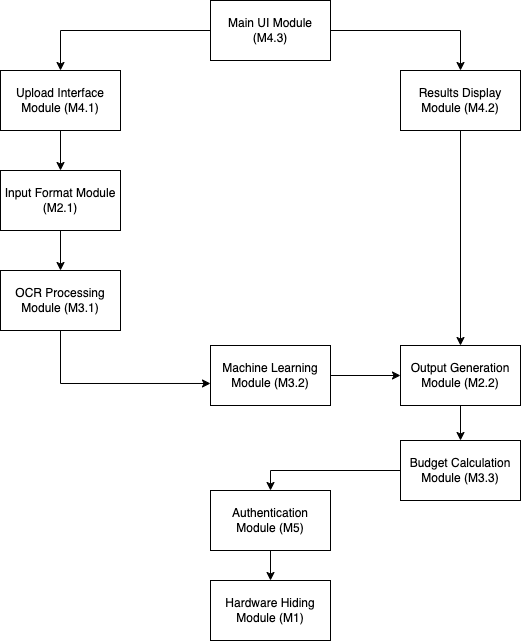
\includegraphics[width=0.7\textwidth]{UsesHierarchy.png}
\caption{Use hierarchy among modules}
\label{FigUH}
\end{figure}

%\section*{References}

\newpage

\section{User Interfaces}

The user interfaces for \textit{Plutos} are prototyped via Figma. All the wire frames are to be translated to front-end code using our programming language of choice (React Native + TypeScript).
The corresponding UI pages can be found down below.
 
\begin{itemize}
	\item \href{https://www.figma.com/design/W2B31TC8L3tgjZm8189vqm/Plutos?node-id=29-45&t=gfR0b4FgWOY40Jt2-1}{User Account Management/Login}.
	\item \href{https://www.figma.com/design/W2B31TC8L3tgjZm8189vqm/Plutos?node-id=112-2933&t=ZbbX5sZyfK6XT3DZ-1}{Add Income/Budget/Expense}.
\end{itemize}

\noindent As \textit{Plutos} is designed to be a fully-functioning app that lives on the cloud, there will be no dedicated hardware components. Hence there are no relevant physical user interfaces.

\section{Design of Communication Protocols}

\begin{enumerate}
	\item \textbf{Overview}: The communication protocol facilitates data exchange between the mobile front end, back-end server, and third-party APIs (e.g., OCR, AI categorization, and external data sources). It ensures secure, reliable, and efficient interactions to enable receipt parsing, expense categorization, and budgeting functionalities.
	\item \textbf{Communication Layers}:
	\begin{itemize}
		\item \textbf{Application Layer}
		\begin{itemize}
			\item \textbf{Purpose}: Handles user-facing operations such as sending images, fetching categorized expenses, and updating budgets.
			\item \textbf{Data Format}: JSON
			\item \textbf{Transport Mechanism}: HTTPS over RESTful API endpoints.
		\end{itemize}
		\item \textbf{Transport Layer}
		\begin{itemize}
			\item \textbf{Protocol}: HTTPS (TLS 1.3 for encryption and secure data transmission).
			\item \textbf{Port}: 443 (Default for HTTPS)
		\end{itemize}
		\item \textbf{Network Layer}
		\begin{itemize}
			\item \textbf{Protocol}: IPv4/IPv6 for data routing and delivery.
			\item \textbf{Fallback Handling}: Automatic retries for intermittent connectivity loss.
		\end{itemize}
	\end{itemize}
	\item \textbf{Data Flow}
	\begin{itemize}
		\item \textbf{Image Upload (Receipt Parsing)}
		\begin{itemize}
			\item \textbf{Front End}:
			\begin{itemize}
				\item Captures the receipt image using the device camera.
				\item Encodes the image in Base64 or uploads as a binary file.
				\item Sends the image along with metadata (e.g., user ID, timestamp) to the back end.
			\end{itemize}
			\item \textbf{Back End}:
			\begin{itemize}
				\item Receives and validates the image payload.
				\item Forwards the image to the OCR/AI service via an internal API call.
			\end{itemize}
		\end{itemize}
		\item \textbf{Expense Categorization}
		\begin{itemize}
			\item \textbf{AI Service}:
			\begin{itemize}
				\item Processes the image and extracts structured data (e.g., items, prices, dates).
				\item Categorizes the extracted data using a machine learning model.
				\item Returns the processed data to the back end.
			\end{itemize}
			\item \textbf{Back End}:
			\begin{itemize}
				\item Formats the categorized data into a JSON response.
				\item Sends it to the front end for user display.
			\end{itemize}
		\end{itemize}
		\item \textbf{Budget and Forecast Management}
		\begin{itemize}
			\item \textbf{Front End}:
			\begin{itemize}
				\item Sends requests for fetching/updating budgets or forecast predictions.
			\end{itemize}
			\item \textbf{Back End}:
			\begin{itemize}
				\item Queries the database for budget/expense data.
				\item Updates user budgets based on inputs.
				\item Runs predictive models for forecasting.
			\end{itemize}
			\item \textbf{Response}:
			\begin{itemize}
				\item Sends updated data or predictions to the front end.
			\end{itemize}
		\end{itemize}
	\end{itemize}
	\newpage
	\item \textbf{API Design}
	\\ \textbf{Endpoints}
	\begin{itemize}
		\item \textbf{POST/upload-receipt}
		\begin{itemize}
			\item \textbf{Request}
			\begin{verbatim}
				{
					"userId": "12345",
					"image": "Base64String or Binary",
					"timestamp": "2025-01-13T10:00:00Z"
				}
			\end{verbatim}
			\item \textbf{Response}
			\begin{verbatim}
				{
					"status": "success",
					"data": {
						"parsedItems": [
							{ "name": "Milk", "price": 3.5, "category": "Groceries" },
							{ "name": "Bread", "price": 2.0, "category": "Groceries" }
						]
					}
				}
			\end{verbatim}
		\end{itemize}
		\item \textbf{GET/expenses}
		\begin{itemize}
			\item \textbf{Request}: \texttt{?userId=12345}
			\item \textbf{Response}:
			\begin{verbatim}
				{
					"status": "success",
					"data": {
						"totalExpenses": 150.75,
						"categories": {
							"Groceries": 75.5,
							"Entertainment": 30.0
						}
					}
				}
			\end{verbatim}
		\end{itemize}
		\item \textbf{PUT/update-budget}
		\begin{itemize}
			\item \textbf{Request}:
			\begin{verbatim}
				{
					"userId": "12345",
					"budget": {
						"Groceries": 200,
						"Entertainment": 100
					}
				}
			\end{verbatim}
			\item \textbf{Response}:
			\begin{verbatim}
				{
					"status": "success",
					"message": "Budget updated successfully."
				}
			\end{verbatim}
		\end{itemize}
	\end{itemize}
	\item \textbf{Error Handling}
	\begin{itemize}
		\item \textbf{HTTP Status Codes}:
		\begin{itemize}
			\item \texttt{200 OK}: Successful operation.
			\item \texttt{400 Bad Request}: Invalid input or missing parameters.
			\item \texttt{401 Unauthorized}: User authentication failed.
			\item \texttt{500 Internal Server Error}: Server-side issues.
		\end{itemize}
		\item \textbf{Error Response Format}:
		\begin{verbatim}
			{
				"status": "error",
				"code": "XXX",
				"message": "Some error code lol idk"
			}
		\end{verbatim}
	\end{itemize}
	\item \textbf{Security Measures}
	\begin{itemize}
		\item \textbf{Authentication and Authorization Using JWT} - To ensure secure communication between the client (mobile app) and the backend server, the system utilizes JWT (JSON Web Token) for authentication and authorization.
		\begin{itemize}
			\item \textbf{Token Generation}
			\begin{itemize}
				\item Upon successful user login or registration, the backend server generates a JWT containing the user's unique identifier (user\_id) and other claims (e.g., roles or permissions) as needed.
				\item The token is signed using a strong secret key or a private key (in the case of asymmetric signing algorithms like RS256) to ensure authenticity.
			\end{itemize}
			\item \textbf{Token Structure}
			\\ A JWT consists of three parts:
			\begin{itemize}
				\item \textbf{Header}: Specifies the signing algorithm (e.g., HS256, RS256).
				\item \textbf{Payload}: Contains claims, such as user information and token expiration (exp).
				\item \textbf{Signature}: Ensures the token has not been tampered with.
			\end{itemize}
			\item \textbf{Token Storage}
			\begin{itemize}
				\item The client stores the JWT securely in memory or a secure storage mechanism (e.g., SecureStore in React Native or AsyncStorage with encryption).
				\item Tokens must never be stored in plain text or local storage to avoid XSS vulnerabilities.
			\end{itemize}
			\item \textbf{Token Validation}
			\begin{itemize}
				\item The backend server validates incoming JWTs in the Authorization header of HTTP requests.
				\\ Example \\
				\texttt{Authorization: Bearer <token>}
				\item Validation includes:
				\begin{itemize}
					\item Verifying the signature.
					\item Checking the exp claim to ensure the token has not expired.
					\item Ensuring the token was issued by a trusted source (iss claim).
				\end{itemize}
			\end{itemize}
			\item \textbf{Token Expiry and Refresh}
			\begin{itemize}
				\item Tokens include a short expiration time (exp) for security.
				\item A \textbf{refresh token} mechanism is implemented to issue new tokens without requiring reauthentication:
				\begin{itemize}
					\item Refresh tokens are stored securely and exchanged only via secure channels (e.g., HTTPS).
					\item When the access token expires, the client uses the refresh token to request a new JWT from the backend.
				\end{itemize}
			\end{itemize}
			\item \textbf{Securing JWT in Transit}
			\begin{itemize}
				\item All API calls using JWT must be encrypted with HTTPS to prevent interception (man-in-the-middle attacks).
				\item Implement strict \textbf{CORS} policies on the backend to prevent unauthorized access.
			\end{itemize}
			\item \textbf{Revocation Mechanisms}
			\begin{itemize}
				\item Implement a blacklist or token revocation strategy to invalidate compromised tokens.
				\item Tokens can be associated with a unique identifier in the database (e.g., a session ID) and marked invalid upon logout or suspected compromise.
			\end{itemize}
		\end{itemize}
	\end{itemize}
\end{enumerate}

\section{Timeline}

A breakdown of the team's delegation of tasks and responsibilities can be found in the respective GitHub repository Issues tab. The
delegation of tasks assumes an even distribution amongst team members as outlined in the \href{https://github.com/PlutosCapstone/Plutos/blob/main/docs/DevelopmentPlan/DevelopmentPlan.pdf}{Development Plan}. However, if situation arises
where a certain task requires additional member's assistance to complete, then the team will need to communicate it across. \\

\noindent All document related issues are to be completed prior to the respective document's Rev1 deadline. This is also the deadline date of the \textit{Final Documentation} . \\

\noindent All feature related issues (functional and non-functional) are to be completed prior to the Rev1 final demonstration. \\

\noindent The link to the GitHub repository Issues tab for \textit{Plutos} can be found \href{https://github.com/PlutosCapstone/Plutos/issues}{here}.

\bibliographystyle {plainnat}
\bibliography{../../../refs/References}

\newpage{}

\end{document}